\documentclass[letterpaper]{article}
\usepackage{cmap}
\usepackage[spanish, mexico, es-nodecimaldot]{babel}
\usepackage{amsmath}
\usepackage{amsthm}
\usepackage{amsfonts}
\usepackage{amssymb}
\usepackage{physics}
% \usepackage{jkmath}
\usepackage{bm}
\usepackage{mathtools}
\usepackage{siunitx}
\usepackage{graphicx}
\usepackage{fancyhdr}
\usepackage{lastpage}
\usepackage{xcolor}
\usepackage{pagecolor}
\usepackage{enumitem}
\usepackage{tasks}
\usepackage{nicefrac}
\usepackage[colorlinks=true]{hyperref}
\usepackage[capitalise]{cleveref}
%%%%%%%%%%%%%%%%%%%%%%%%%%%%%%%%%%%%%%%%%%%%%%%%%%%%%%%%%%%%%%%!
%%%%* Configuraciones adicionales del documento
\newcommand{\Titletarea}{Repaso de mecánica newtoniana}
\newcommand{\Clase}{Mecánica Analítica}
\definecolor{base3}{RGB}{253, 246, 227}%
\pagecolor{base3}
\sisetup{
    per-mode=symbol-or-fraction,
    range-phrase=~a~
}
\graphicspath{{Figuras/}}
\topmargin=-1.5cm
\evensidemargin=0in
\oddsidemargin=0in
\textwidth=6.5in
\textheight=9.5in
\headsep=0.25in

\linespread{1.1}

\pagestyle{fancy}
\lhead{Grupo 8198, Sem. 2021-2}
\chead{\Clase}
\rhead{\Titletarea}
% \lfoot{\today}
\cfoot{\textbf{Facultad de Ciencias, UNAM}}
\rfoot{Página \thepage \hspace{1pt} de \pageref{LastPage}}
\renewcommand\headrulewidth{0.4pt}
\renewcommand\footrulewidth{0.4pt}
\setlength\parindent{0pt}

\hypersetup{
    linkcolor={[rgb]{0,0.2,0.6}},
    citecolor={[rgb]{0,0.6,0.2}},
    filecolor={[rgb]{0.8,0,0.8}},
    urlcolor={[rgb]{0.8,0,0.8}},
    runcolor={[rgb]{0.8,0,0.8}},  
    menucolor={[rgb]{0,0.2,0.6}},
    linkbordercolor={[rgb]{0,0.2,0.6}},
    citebordercolor={[rgb]{0,0.6,0.2}},
    filebordercolor={[rgb]{0.8,0,0.8}},
    urlbordercolor={[rgb]{0.8,0,0.8}},
    runbordercolor={[rgb]{0.8,0,0.8}},
    menubordercolor={[rgb]{0,0.2,0.6}}, 
    pdftitle={Tarea},%
    pdfauthor={Autor(es)},%
    pdfsubject={Mecánica Analítica},%
    pdfkeywords={Palabras clave}
}
%%%%%%%%%%%%%%%%%%%%%%%%%%%%%%%%%%%%%%%%%%%%%%%%%%%%%%%%%%%%%%%!
%%%%* Portada


\title{
    \vspace{-1.5cm}
    \textbf{Tarea 1:\ \Titletarea}\\
    \normalsize\vspace{0.1in}\small{\textbf{Entrega}:~\today}\\
    \vspace{0.1in}\large{Prof.: Dr. Fermín Viniegra Heberlein\\
    \; Prof.: Fís. Jonathan Urrutia Anguiano\\
    \ Ayud.: José Samuel Rodríguez Olguín\\
    \ Ayud.: Isabel Yajaira Rojas Martinez}
    \vspace{0.5cm}
}
\author{
    Apellidos1, Nombres1
    \and
    Apellidos2, Nombres2
    \and 
    Apellidos3, Nombres3
    \and 
    Apellidos4, Nombres4
}
\date{}

%%%%* Comandos útiles
\newcommand{\solution}{\textbf{\large Solución}\\}
%\crefname{table}{\textbf{Tabla}}{\textbf{Tablas}}
%\crefname{equation}{\textbf{ec.}}{\textbf{ecuaciones}}
%\crefname{figure}{\textbf{Fig.}}{\textbf{Figuras}}
\newcommand\crefrangeconjunction{{}--{}}
\newcommand\crefpairconjunction{ y }
\newcommand{\salirmodo}{\leavevmode \\}
\setlength{\jot}{10pt}
\newcommand*\Eval[3]{\left.#1\right\rvert_{#2}^{#3}}
\newcommand{\QfuckingED}{\qed}
\renewcommand\qedsymbol{\(\blacksquare\)}
\newcommand{\uveci}{{\bm{\hat{\textnormal{\bfseries\i}}}}}
\newcommand{\uvecj}{{\bm{\hat{\textnormal{\bfseries\j}}}}}
\DeclareRobustCommand{\uvec}[1]{{%
  \ifcsname uvec#1\endcsname
     \csname uvec#1\endcsname
   \else
    \bm{\hat{\mathbf{#1}}}%
   \fi
}}
\newcommand{\idest}{\textbf{i.e.,}~}

\begin{document}
\maketitle
\thispagestyle{fancy}
\section*{Análisis de fuerzas}
\begin{enumerate}[label=\textbf{1.\arabic*)}]
    \item \textbf{Leyes de Newton:}\salirmodo
    Un hombre empuja un carrito del supermercado con una mano, y el carrito, inicialmente en reposo, comienza a moverse. Entonces, la mano debe estar ejerciendo una fuerza sobre el carro. Por la tercera ley de Newton, el carro debe estar ejerciendo una fuerza sobre su mano en la dirección opuesta de misma magnitud. ¿Cómo puede ser esto posible, si su mano obviamente no se está acelerando en la dirección contraria? \\
    Justifique su respuesta.
    \item \textbf{Sistemas no inerciales}\salirmodo
    Uno de los cachorros de Lilia, de masa \(m\), se sienta en un carrusel a una distancia \(r\) de su centro. Un niño da impulso al carrusel de tal forma que gira a una velocidad \(\bm{\omega}=\omega\uvec{e}_{z}\). El coeficiente de fricción estática entre el carrusel y las patitas del cachorro es de \(\mu\).
\begin{itemize}[label = \textbullet]
    \item Haz el diagrama de cuerpo libre del cachorro montado en el sistema del carrusel.
    \item Escribe las ecuaciones de movimiento del bloque con base en el inciso anterior.
    \item Determina el radio máximo \(R\) en el cual el perrito permanece en reposo respecto al sistema del carrusel (es decir, el radio máximo para el que no hay forma que se caiga el perrito y se lastime).
\end{itemize}
    \item \textbf{Máquina de Atwood doble:}\salirmodo
    Considera dos cachorros de masa \(m_{1}\) y \(m_{2}\) unidos por un lazo que cuelga de una polea; tanto la polea como el lazo tienen masa despreciable y la polea también tiene tamaño despreciable. A su vez, esta polea está unida, por otro lazo, a otro cachorro con masa \(m_{3}\); nuevamente el tamaño de la polea y la masa de ésta y del lazo son despreciables.
    \begin{itemize}[label = \textbullet]
        \item Haz el diagrama de fuerzas sobre los tres cachorros
        \item Escribe las ecuaciones de movimiento para cada perrito y resuélvelas.
        \item Identifica los casos en los que los cachorros se mantienen estáticos.
    \end{itemize}
    Para visualizar este efecto y corroborar tu solución puedes apoyarte con \url{https://demonstrations.wolfram.com/DoubleAtwoodMachine/}
    \begin{figure}[htb]
        \centering
        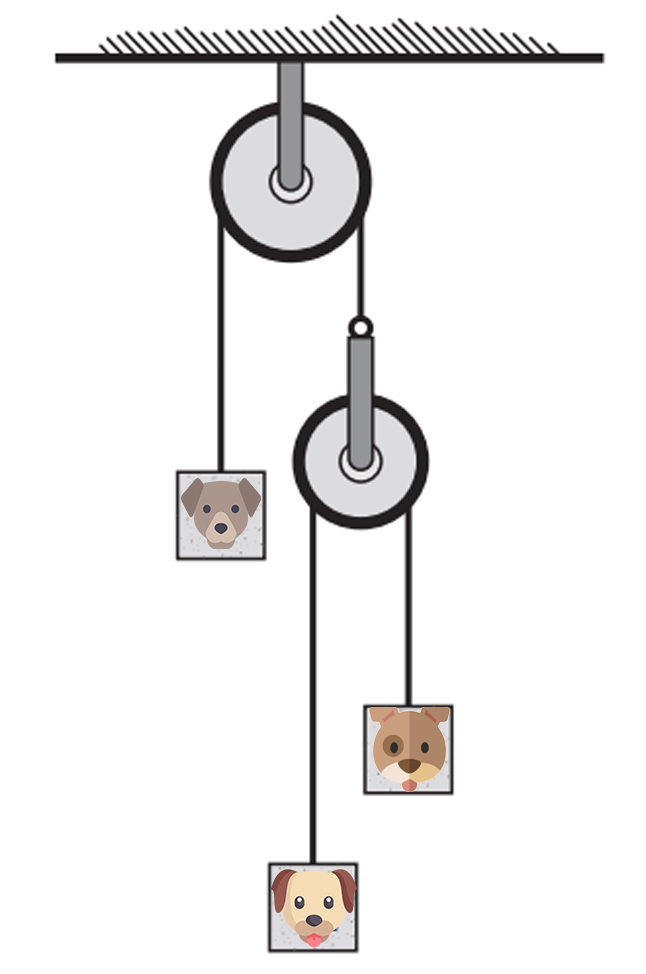
\includegraphics[width=0.35\textwidth]{AtwoodPerros.png}
        \caption{\footnotesize Esquema de una máquina de Atwood doble; una polea sujeta al techo carga a un cachorro y a una segunda polea que, a su vez, sostiene a dos cachorros más. Ambas poleas tienen tamaño despreciable y sus masas, como las de la cuerdas, también son despreciables.} 
    \end{figure}
    \pagebreak
    \item Supongase que una regla lisa de madera de masa \(m\) está en equilibrio sostenida por dos dedos a diferentes distancias \(a\) y \(b\) de su punto medio (ver \cref{fig:regla}).	Sea \(\mu\) el coeficiente de fricción cinética de la madera con los dedos, y \(\mu_{s}\) el coeficiente de fricción estática. En general, se tiene la relación \(\mu \leq \mu_{s}\), aunque en muchos casos se cumple \(\mu <\mu_{s}\); este es el caso de la madera sobre los dedos.
	\begin{itemize}[label = \textbullet]
		\item Las fuerzas en \(A\) y \(B\) son \(\vb{F}_{A}=\nicefrac{mgb}{(a+b)}\) y \(\vb{F}_{B}=\nicefrac{mgb}{(a+b)}\). 	Asumiendo que \(b>a\), como en la \cref{fig:regla}, se tiene que \(\norm{\vb{F}_{A}}>\norm{\vb{F}_B}\).\\
		Muestra que, cuando los dedos se acercan el uno al otro, \(A\) permanece en la misma posición en la regla mientras que \(B\) se mueve a una distancia \(b_{1}<a\), donde la fricción cinética de \(B\) es igual a la fricción estática de \(A\), y por lo tanto \(\mu a=\mu_{s} b_{1}\) y \(\frac{a}{b_{1}}=\mu_{s}/\mu>1\).
		\item En este punto, \(A\) empieza a moverse hasta que se cumpla la relación \(b_{1}/{a_{1}}={\mu_{s}}/{\mu}\).	Muestre que, de esta manera, \(A\) y \(B\) se aproximan entre ellos con una progresión geométrica hasta que estos lleguen al punto medio. 
	\end{itemize}
    \begin{figure}[htb]
        \centering
        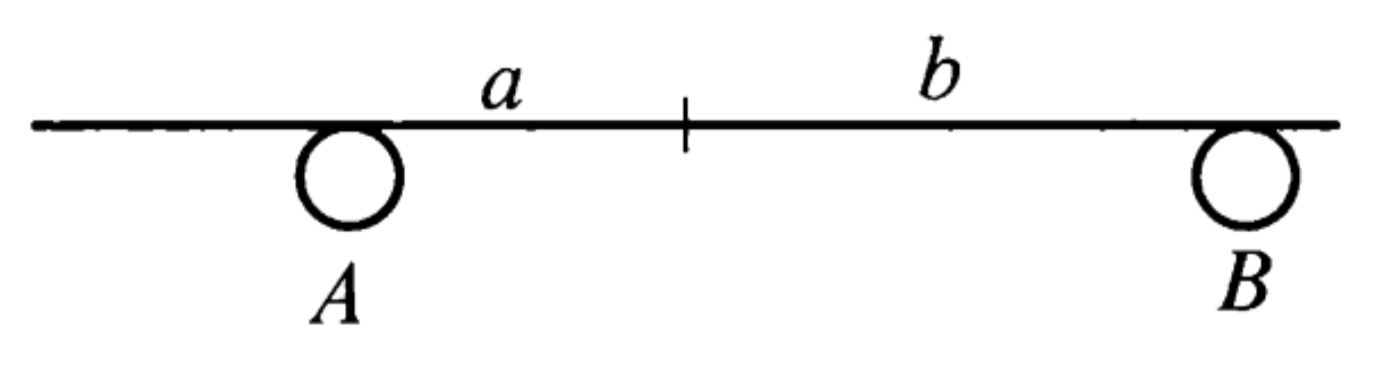
\includegraphics[width=0.6\textwidth]{imagen3.png}
        \caption{\footnotesize Diagrama de la regla de madera (línea horizontal) y los dedos (círculos) en las posiciones \(A\) y \(B\) alejados del centro de masa de la regla a una distancia \(a\) y \(b\), respectivamente.}
        \label{fig:regla}
    \end{figure}
\end{enumerate}
\section*{Energía}
\begin{enumerate}[label=\textbf{2.\arabic*)}]
    \setcounter{enumi}{4}
    \item Se dice que una fuerza \(\vb{F}\) es conservativa si el trabajo que realiza es independiente de la trayectoria de integración, es decir que
    \begin{equation*}
        W = \oint \vb{F}\vdot \dd{\bm{\ell}} = 0.
    \end{equation*}
    Escribe otras dos equivalencias de la definición anterior.\salirmodo
    \item Un objeto de masa \(M\) en reposo explota y se fragmenta en dos pedazos de masa \(m_{1}\) y \(m_{2}\) de tal forma que \(M = m_{1}+m_{2}\). En la explosión se libera una cantidad de energía \(Q\).
    \begin{itemize}[label = \textbullet]
        \item ¿Cuál es la energía cinética de cada fragmento después de la explosión?
        \item ¿Qué porcentaje de la energía total liberada recibirá cada fragmento si \(m_{1} = 4 m_{2}\)?
    \end{itemize}
    \salirmodo
    \item Una partícula de masa m se mueve a lo largo del eje \(x\) bajo la influencia de una fuerza conservativa de potencial \(V(x)\). Si la partícula se encuentra en las posiciones \(x_{1}\) y \(x_{2}\) a tiempos \(t_{1}\) y \(t_{2}\), probar que si E es la energía total:
    \begin{align*}
        t_{2}-t_{1}=\sqrt{\frac{m}{2}}\int\displaylimits_{x_{1}}^{x_{2}}\frac{\dd{x}}{\sqrt{E-V(x)}}.
    \end{align*}\salirmodo
\end{enumerate}
\section*{Ecuaciones diferenciales}
\begin{enumerate}[label={\textbf{3.\arabic*)}}]
    \setcounter{enumi}{7}
    \item La ecuación de un movimiento oscilatorio puede, en general, escribirse como
    \begin{align*}
       m \ddot{x} + \gamma \dot{x} + m\omega_{0}^{2}x = 0,
    \end{align*}
    donde \(m\) es la masa del objeto, \(\gamma\) es una constante de amortiguamiento y \(\omega_{0}^{2}\) es la frecuencia natural del sistema oscilatorio. Resuelve la ecuación diferencial y, proponiendo condiciones iniciales razonables, analiza los siguientes casos:
    \begin{tasks}(4)
        \task \(\gamma = 0\),
        \task \(\omega_{0}^{2}>(\gamma/2)^{2}\),
        \task \(\omega_{0}^{2}<(\gamma/2)^{2}\),
        \task \(\omega_{0}^{2}=(\gamma/2)^{2}\).
    \end{tasks}
    \textit{Hint:} Una forma de resolver la ecuación diferencial es proponiendo una solución del tipo \(x(t)= x_{0}e^{\lambda t}\) y ver qué debe cumplir \(\lambda\).\salirmodo
    \item \textbf{Velocidad terminal:}\\
    Considera el caso de caída libre unidimensional pero introduce un término de fricción que sea proporcional a la velocidad; al igual que en el inciso anterior este es un término disipativo.
    \begin{itemize}[label = \textbullet]
    \item  Si tenemos las condiciones iniciales \(y(t=0) = h\) y \(\dot{y}(t=0) = 0\), determina la velocidad máxima que alcanza el objeto que cae.
    \item Compara la ecuación diferencial de este inciso con la anterior. ¿Son muy diferentes?
    \end{itemize}\salirmodo
\end{enumerate}
\end{document} 